\subsection {Session 6, Exercise 5}

\label{6_5}

\lineparagraph {Exercise}

Give a Turing-machine for the language

\begin{align*}
 L = \{w\#w | w \in{} \{0,1\}^*\}.
\end{align*}

Give an upper bound for the running time.

\lineparagraph {Solution}

This is the Turing-machine:

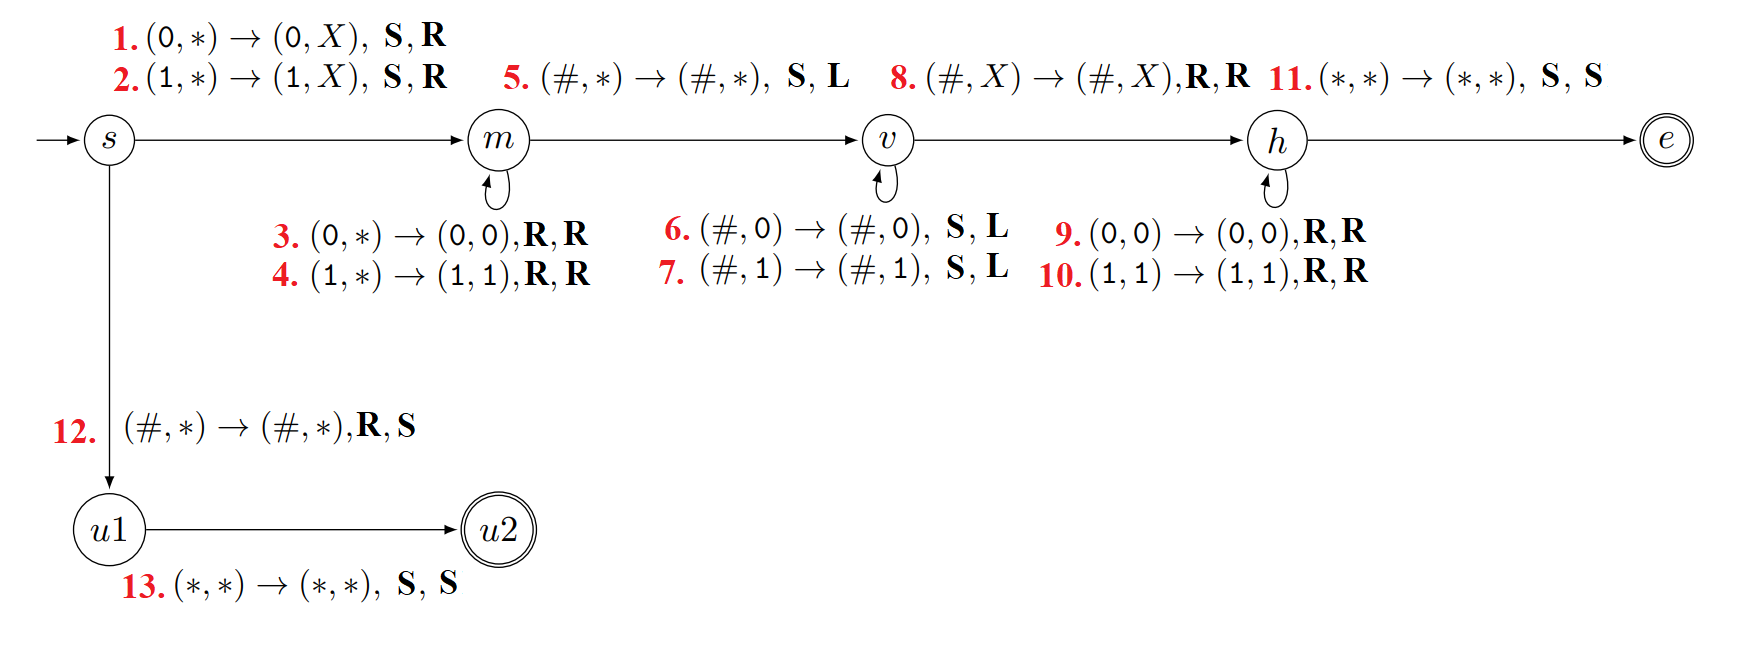
\includegraphics[width=\linewidth]{06/6_5.png}

Proof: This machine's language is $L$.

States and transitions:
\begin{itemize}
    \item State $s$: The starting state, the empty string will remain here.
    \item Transitions $1$ and $2$: will put an $X$ at the beginning of the second tape, for protection against failling off.
    \item State $m$: Used for copying the input word up until the first $\#$ to the second tape.
    \item Transitions 3-4: Copy a $0$ or a $1$ to the second tape, move both heads to the next position.
    \item Transition 5: When we encounter the first $\#$ we stop copying and move to state $v$, while positioning the second head back to the last copied character. If there is no $\#$ in the word the computation halts in state $m$ and rejects the input correctly.
    \item State $v$: Used for moving the second head back to the beginning of the second tape.
    \item Transitions 6-7: The first head will stay on the character $\#$, while the second head moves to the left while it sees a $0$ or a $1$.
    \item Transition 8: When the second head sees the $X$ at the beginning of the second tape it reached the beginning of the tape. The heads are positioned, so the first head is at the beginning of the (copied) input, while the second head is at the first character after the $\#$ in the input.
    \item State $h$: Used to compare the first part of the input (before the $\#$) to the second part of the input (after the $\#$).
    \item Transitions 9-10: We make sure that all characters match in the fist and the second part of the inputa word, so that it is in $w\#w$ form.
    \item Transition 11: Only allows moving to the accepting $e$ state if the the two heads reach the empty cells at the same time = if the two parts of the input word match. If the word contains another $\#$, or if the two parts don't match, then this transition won't be able to fire and we won't be able to move to state $e$.
    \item State $e$: Only words in the language can reach this state to accept. No further computation needed.
    \item Transition 12: There is a special word, $\#$, which the generic computation above cannot handle, since it has no $0$ or $1$ characters, however it should be accepted, since $w$ is allowed to be the empty string. We handle this case specially, we detect that on the input we see the $\#$ character, and
    \item Transition 13: Detects that there is no further characters in the input, so the input word is $\#$ exactly.
    \item States $u1$ and $u2$: Used for handling this special case, $u2$ will accept the $\#$ only.
\end{itemize}

Accepting / rejecting states, accepted / rejected words:

\begin{itemize}
    \item If the word starts with $\#$ character it is moved to $u1$. It can only be accepted if the word is $\#$ exactly, no further characters can come. $\#$ is moved to $u2$ and accepted, while the others remain in $u1$ and get rejected there.
    \item If the word starts with some $0$ or $1$ characters, those get copied to the second tape.
    \item If the word contains no $\#$ character then it stops in state $m$ and gets rejected.
    \item If the word contains a $\#$ character, the characters coming after should match what characters were before. So any word in the form $w\#w$ is accepted, however any $w\#h$, where $w\neq{}h$ will stop in state $h$ and will be rejected. This includes the words that contain more $\#$'s (in $h$) and words that contain only $0$'s and $1$'s in $h$, but not match $w$, since the only possible way to activate transition 11 is to have matching characters before the $\#$ and after it. State $e$ accepts these words.
\end{itemize}

Upper bound for the running time: the longest running time will be an accepted word that reachers state $e$. If the word is $w\#w$, of lenght $n=2k+1$, so that $w$ is of length $k$, then:

\begin{itemize}
    \item Transitions 1-2: $1$ step, to put down an $X$.
    \item Transitions 3-4: $k$ steps, to copy $w$ to the second tape.
    \item Transition 5: $1$ step to detect the $\#$ and position.
    \item Transitions 6-7: $k$ steps to move the second head to the first position on the second tape.
    \item Transition 8: $1$ step to detect the beginning of the second tape and position the heads.
    \item Transitions 9-10: $k$ steps to compare the two parts.
    \item Transition 11: $1$ step to see that they end at the same time.
\end{itemize}

$1+k+1+k+1+k+1 = 3k+4$ steps, where $n=2k+1$, so $k=\frac{n}{2}-1$, so $3k+4 = 3(\frac{n}{2}-1)+4 = \frac{3n}{2}+1 \in{} O(n)$. For accepted words this is $\Theta(n)$, for rejected words not necessarily, for example the input word $\#0^k$, for any large $k$ will be rejected after $1$ step, in $u1$.